%
% Documento: Apêndices
%

\begin{apendicesenv}
\partapendices

\lstset{
	frame=single,
    breaklines=true,
    language=HTML
    }
    
\chapter{Código de teste para a técnica ''Faça menos requisições HTTP'': Arquivos Separados}
\label{apend:codigo_facamenosrequisicoeshttp_sep}

\begin{lstlisting}
<!DOCTYPE html>
<html>
<head>
<link rel=''stylesheet'' href=''css/animate.css''>
<link rel=''stylesheet'' href=''css/bootstrap.min.css''>
<link rel=''stylesheet'' href=''css/bootstrap-theme.min.css''>
<link rel=''stylesheet'' href=''css/font-awesome.min.css''>
<link rel=''stylesheet'' href=''css/fullcalendar.min.css''>
<link rel=''stylesheet'' href=''css/normalize.css''>
<link rel=''stylesheet'' href=''css/skeleton.css''>
	
<link rel=''stylesheet'' href=''css/animate - Copy.css''>
<link rel=''stylesheet'' href=''css/bootstrap.min - Copy.css''>
<link rel=''stylesheet'' href=''css/bootstrap-theme.min - Copy.css''>
<link rel=''stylesheet'' href=''css/font-awesome.min - Copy.css''>
<link rel=''stylesheet'' href=''css/fullcalendar.min - Copy.css''>
<link rel=''stylesheet'' href=''css/normalize - Copy.css''>
<link rel=''stylesheet'' href=''css/skeleton - Copy.css''>
</head>

<body>

<h1>My First Heading</h1>

<p>My first paragraph.</p>

<img src=''imgs/1.jpg'' />
<img src=''imgs/2.jpg'' />
<img src=''imgs/3.jpg'' />
<img src=''imgs/4.jpg'' />
<img src=''imgs/5.jpg'' />
<img src=''imgs/6.jpg'' />
<img src=''imgs/7.jpg'' />
<img src=''imgs/8.jpg'' />
<img src=''imgs/9.jpg'' />
<img src=''imgs/10.jpg'' />
<img src=''imgs/11.jpg'' />
<img src=''imgs/12.jpg'' />
<img src=''imgs/13.jpg'' />
<img src=''imgs/14.png'' />
<img src=''imgs/15.png'' />
<img src=''imgs/16.jpg'' />
<img src=''imgs/17.jpg'' />
<img src=''imgs/18.jpg'' />
<img src=''imgs/19.jpg'' />
<img src=''imgs/20.jpg'' />
<img src=''imgs/21.jpg'' />
<img src=''imgs/22.jpg'' />
<img src=''imgs/23.jpg'' />
<img src=''imgs/24.jpg'' />
<img src=''imgs/25.jpg'' />
<img src=''imgs/26.jpg'' />
<img src=''imgs/27.jpg'' />
<img src=''imgs/28.jpg'' />
	

<script src=''js/jquery-2.1.4.min.js''></script>
<script src=''js/angular.min.js''></script>
<script src=''js/backbone.js''></script>
<script src=''js/bootstrap.min.js''></script>
<script src=''js/d3.min.js''></script>
<script src=''js/ember-data.min.js''></script>
<script src=''js/fullcalendar.min.js''></script>
<script src=''js/highcharts.js''></script>
<script src=''js/moment-with-locales.min.js''></script>
<script src=''js/require.js''></script>
</body>
</html>
\end{lstlisting}

\chapter{Código de teste para a técnica ''Faça menos requisições HTTP'': Arquivos Concatenados}
\label{apend:codigo_facamenosrequisicoeshttp_concat}

\begin{lstlisting}
<!DOCTYPE html>
<html>
<head>
<link rel=''stylesheet'' href=''css/minified.css''>
</head>

<body>

<h1>My First Heading</h1>
<p>My first paragraph.</p>
	
<img src=''imgs/1.jpg'' />
<img src=''imgs/2.jpg'' />
<img src=''imgs/3.jpg'' />
<img src=''imgs/4.jpg'' />
<img src=''imgs/5.jpg'' />
<img src=''imgs/6.jpg'' />
<img src=''imgs/7.jpg'' />
<img src=''imgs/8.jpg'' />
<img src=''imgs/9.jpg'' />
<img src=''imgs/10.jpg'' />
<img src=''imgs/11.jpg'' />
<img src=''imgs/12.jpg'' />
<img src=''imgs/13.jpg'' />
<img src=''imgs/14.png'' />
<img src=''imgs/15.png'' />
<img src=''imgs/16.jpg'' />
<img src=''imgs/17.jpg'' />
<img src=''imgs/18.jpg'' />
<img src=''imgs/19.jpg'' />
<img src=''imgs/20.jpg'' />
<img src=''imgs/21.jpg'' />
<img src=''imgs/22.jpg'' />
<img src=''imgs/23.jpg'' />
<img src=''imgs/24.jpg'' />
<img src=''imgs/25.jpg'' />
<img src=''imgs/26.jpg'' />
<img src=''imgs/27.jpg'' />
<img src=''imgs/28.jpg'' />

	<script src=''js/minified.js''></script>
</body>
</html>

\end{lstlisting}

\chapter{Código de teste para a técnica ''Reduza o número de pesquisas DNS'': Multiplas CDN}
\label{apend:codigo_reduzaonumerodepesquisasdns_mult}	

\begin{lstlisting}
<!DOCTYPE html>
<html>
<head>
<link rel=''stylesheet'' href=''//cdnjs.cloudflare.com/ajax/libs/animate.css/3.4.0/animate.min.css''>
<link rel=''stylesheet'' href=''//maxcdn.bootstrapcdn.com/bootstrap/3.3.5/css/bootstrap.min.css''>
<link rel=''stylesheet'' href=''//maxcdn.bootstrapcdn.com/font-awesome/4.4.0/css/font-awesome.min.css''>	
<link rel=''stylesheet'' href=''//cdnjs.cloudflare.com/ajax/libs/fullcalendar/2.0.2/fullcalendar.js''>
<link rel=''stylesheet'' href=''//cdn.bootcss.com/skeleton/2.0.4/skeleton.css''>
<link rel=''stylesheet'' href=''css/normalize.css''>
</head>

<body>

<h1>My First Heading</h1>
<p>My first paragraph.</p>

<img src=''imgs/1.jpg'' />
<img src=''imgs/2.jpg'' />
<img src=''imgs/3.jpg'' />
<img src=''imgs/4.jpg'' />
<img src=''imgs/5.jpg'' />
<img src=''imgs/6.jpg'' />
<img src=''imgs/7.jpg'' />
<img src=''imgs/8.jpg'' />
<img src=''imgs/9.jpg'' />
<img src=''imgs/10.jpg'' />
<img src=''imgs/11.jpg'' />
<img src=''imgs/12.jpg'' />
<img src=''imgs/13.jpg'' />
<img src=''imgs/14.png'' />
<img src=''imgs/15.png'' />
<img src=''imgs/16.jpg'' />
<img src=''imgs/17.jpg'' />
<img src=''imgs/18.jpg'' />
<img src=''imgs/19.jpg'' />
<img src=''imgs/20.jpg'' />
<img src=''imgs/21.jpg'' />
<img src=''imgs/22.jpg'' />
<img src=''imgs/23.jpg'' />
<img src=''imgs/24.jpg'' />
<img src=''imgs/25.jpg'' />
<img src=''imgs/26.jpg'' />
<img src=''imgs/27.jpg'' />
<img src=''imgs/28.jpg'' />

<script src=''//ajax.googleapis.com/ajax/libs/jquery/2.1.4/jquery.min.js''></script>
<script src=''//maxcdn.bootstrapcdn.com/bootstrap/3.3.5/js/bootstrap.min.js''></script>
<script src=''//ajax.googleapis.com/ajax/libs/angularjs/1.3.14/angular.min.js''></script>
<script src=''//cdnjs.cloudflare.com/ajax/libs/d3/3.5.6/d3.js''></script>
<script src=''//cdn.bootcss.com/ember.js/2.1.0-beta.2/ember.js''></script>
<script src=''js/require.js''></script>	
</body>
</html>

\end{lstlisting}

\chapter{Código de teste para a técnica ''Reduza o número de pesquisas DNS'': Única CDN}
\label{apend:codigo_reduzaonumerodepesquisasdns_unic}	

\begin{lstlisting}
<!DOCTYPE html>
<html>
<head>
<link rel=''stylesheet'' href=''//cdnjs.cloudflare.com/ajax/libs/animate.css/3.4.0/animate.min.css''>
<link rel=''stylesheet'' href=''//cdnjs.cloudflare.com/ajax/libs/twitter-bootstrap/4.0.0-alpha/js/bootstrap.min.js''>
<link rel=''stylesheet'' href=''//cdnjs.cloudflare.com/ajax/libs/font-awesome/4.4.0/css/font-awesome.min.css''>	
<link rel=''stylesheet'' href=''//cdnjs.cloudflare.com/ajax/libs/fullcalendar/2.0.2/fullcalendar.js''>
<link rel=''stylesheet'' href=''//cdnjs.cloudflare.com/ajax/libs/skeleton/2.0.4/skeleton.css''>
<link rel=''stylesheet'' href=''//cdnjs.cloudflare.com/ajax/libs/normalize/3.0.3/normalize.css''>
</head>

<body>

<h1>My First Heading</h1>
<p>My first paragraph.</p>

<img src=''imgs/1.jpg'' />
<img src=''imgs/2.jpg'' />
<img src=''imgs/3.jpg'' />
<img src=''imgs/4.jpg'' />
<img src=''imgs/5.jpg'' />
<img src=''imgs/6.jpg'' />
<img src=''imgs/7.jpg'' />
<img src=''imgs/8.jpg'' />
<img src=''imgs/9.jpg'' />
<img src=''imgs/10.jpg'' />
<img src=''imgs/11.jpg'' />
<img src=''imgs/12.jpg'' />
<img src=''imgs/13.jpg'' />
<img src=''imgs/14.png'' />
<img src=''imgs/15.png'' />
<img src=''imgs/16.jpg'' />
<img src=''imgs/17.jpg'' />
<img src=''imgs/18.jpg'' />
<img src=''imgs/19.jpg'' />
<img src=''imgs/20.jpg'' />
<img src=''imgs/21.jpg'' />
<img src=''imgs/22.jpg'' />
<img src=''imgs/23.jpg'' />
<img src=''imgs/24.jpg'' />
<img src=''imgs/25.jpg'' />
<img src=''imgs/26.jpg'' />
<img src=''imgs/27.jpg'' />
<img src=''imgs/28.jpg'' />

<script src=''//cdnjs.cloudflare.com/ajax/libs/jquery/2.1.4/jquery.min.js''></script>
<script src=''//cdnjs.cloudflare.com/ajax/libs/twitter-bootstrap/3.3.5/js/bootstrap.min.js''></script>
<script src=''//cdnjs.cloudflare.com/ajax/libs/angular.js/1.3.14/angular.min.js''></script>
<script src=''//cdnjs.cloudflare.com/ajax/libs/d3/3.5.6/d3.js''></script>
<script src=''//cdnjs.cloudflare.com/ajax/libs/ember.js/2.1.0-beta.2/ember.js''></script>
<script src=''//cdnjs.cloudflare.com/ajax/libs/require.js/2.1.20/require.min.js''></script>	
</body>
</html>

\end{lstlisting}

\chapter{Código de teste para a técnica ''Quebrando domínios dominantes''}
\label{apend:quebrandodominiodominantes}

Para duas CDNs
\begin{lstlisting}
<!DOCTYPE html>
<html>
<head>
<link rel=''stylesheet'' href=''//cdnjs.cloudflare.com/ajax/libs/animate.css/3.4.0/animate.min.css''>
<link rel=''stylesheet'' href=''//maxcdn.bootstrapcdn.com/bootstrap/3.3.5/css/bootstrap.min.css''>
<link rel=''stylesheet'' href=''//maxcdn.bootstrapcdn.com/font-awesome/4.4.0/css/font-awesome.min.css''>	
<link rel=''stylesheet'' href=''//cdnjs.cloudflare.com/ajax/libs/fullcalendar/2.0.2/fullcalendar.js''>
<link rel=''stylesheet'' href=''//cdnjs.cloudflare.com/ajax/libs/skeleton/2.0.4/skeleton.css''>
<link rel=''stylesheet'' href=''//cdnjs.cloudflare.com/ajax/libs/normalize/3.0.2/normalize.css''>
</head>

<body>

<h1>My First Heading</h1>
<p>My first paragraph.</p>
	
<img src=''imgs/1.jpg'' />
<img src=''imgs/2.jpg'' />
<img src=''imgs/3.jpg'' />
<img src=''imgs/4.jpg'' />
<img src=''imgs/5.jpg'' />
<img src=''imgs/6.jpg'' />
<img src=''imgs/7.jpg'' />
<img src=''imgs/8.jpg'' />
<img src=''imgs/9.jpg'' />
<img src=''imgs/10.jpg'' />
<img src=''imgs/11.jpg'' />
<img src=''imgs/12.jpg'' />
<img src=''imgs/13.jpg'' />
<img src=''imgs/14.png'' />
<img src=''imgs/15.png'' />
<img src=''imgs/16.jpg'' />
<img src=''imgs/17.jpg'' />
<img src=''imgs/18.jpg'' />
<img src=''imgs/19.jpg'' />
<img src=''imgs/20.jpg'' />
<img src=''imgs/21.jpg'' />
<img src=''imgs/22.jpg'' />
<img src=''imgs/23.jpg'' />
<img src=''imgs/24.jpg'' />
<img src=''imgs/25.jpg'' />
<img src=''imgs/26.jpg'' />
<img src=''imgs/27.jpg'' />
<img src=''imgs/28.jpg'' />

<script src=''//cdnjs.cloudflare.com/ajax/libs/jquery/2.1.4/jquery.min.js''></script>
<script src=''//maxcdn.bootstrapcdn.com/bootstrap/3.3.5/js/bootstrap.min.js''></script>
<script src=''//cdnjs.cloudflare.com/ajax/libs/angular.js/1.3.14/angular.min.js''></script>
<script src=''//cdnjs.cloudflare.com/ajax/libs/d3/3.5.6/d3.js''></script>
<script src=''//cdnjs.cloudflare.com/ajax/libs/ember.js/2.1.0-beta.2/ember.js''></script>
<script src=''//cdnjs.cloudflare.com/ajax/libs/require.js/2.1.20/require.min.js''></script>	
</body>
</html>
\end{lstlisting}

Para três CDNs
\begin{lstlisting}
<!DOCTYPE html>
<html>
<head>
<link rel=''stylesheet'' href=''//cdnjs.cloudflare.com/ajax/libs/animate.css/3.4.0/animate.min.css''>
<link rel=''stylesheet'' href=''//maxcdn.bootstrapcdn.com/bootstrap/3.3.5/css/bootstrap.min.css''>
<link rel=''stylesheet'' href=''//maxcdn.bootstrapcdn.com/font-awesome/4.4.0/css/font-awesome.min.css''>	
<link rel=''stylesheet'' href=''//cdnjs.cloudflare.com/ajax/libs/fullcalendar/2.0.2/fullcalendar.js''>
<link rel=''stylesheet'' href=''//cdn.bootcss.com/skeleton/2.0.4/skeleton.css''>
<link rel=''stylesheet'' href=''//cdnjs.cloudflare.com/ajax/libs/normalize/3.0.2/normalize.css''>
</head>

<body>

<h1>My First Heading</h1>
<p>My first paragraph.</p>
	
<img src=''imgs/1.jpg'' />
<img src=''imgs/2.jpg'' />
<img src=''imgs/3.jpg'' />
<img src=''imgs/4.jpg'' />
<img src=''imgs/5.jpg'' />
<img src=''imgs/6.jpg'' />
<img src=''imgs/7.jpg'' />
<img src=''imgs/8.jpg'' />
<img src=''imgs/9.jpg'' />
<img src=''imgs/10.jpg'' />
<img src=''imgs/11.jpg'' />
<img src=''imgs/12.jpg'' />
<img src=''imgs/13.jpg'' />
<img src=''imgs/14.png'' />
<img src=''imgs/15.png'' />
<img src=''imgs/16.jpg'' />
<img src=''imgs/17.jpg'' />
<img src=''imgs/18.jpg'' />
<img src=''imgs/19.jpg'' />
<img src=''imgs/20.jpg'' />
<img src=''imgs/21.jpg'' />
<img src=''imgs/22.jpg'' />
<img src=''imgs/23.jpg'' />
<img src=''imgs/24.jpg'' />
<img src=''imgs/25.jpg'' />
<img src=''imgs/26.jpg'' />
<img src=''imgs/27.jpg'' />
<img src=''imgs/28.jpg'' />

<script src=''//cdn.bootcss.com/jquery/2.1.4/jquery.min.js''></script>
<script src=''//maxcdn.bootstrapcdn.com/bootstrap/3.3.5/js/bootstrap.min.js''></script>
<script src=''//cdn.bootcss.com/angular.js/1.3.4/angular.min.js''></script>
<script src=''//cdnjs.cloudflare.com/ajax/libs/d3/3.5.6/d3.js''></script>
<script src=''//cdn.bootcss.com/ember.js/2.1.0-beta.2/ember.js''></script>
<script src=''//cdn.bootcss.com/require.js/2.1.20/require.min.js''></script>	
</body>
</html>

\end{lstlisting}

\chapter{Configurando \textit{nghttp2}}
\label{apend:configurandonghttp2}

Apesar de descrita no site oficial do projeto\footnote{https://github.com/tatsuhiro-t/nghttp2}, a configuração do \textit{nghttp2} só foi possível graças a \citeonline{nghttp2config}. Em seu artigo Tollman descreve bem detalhadamente o processo de instalação do \textit{nghttp2} e suas dependências. Enquanto que no site oficial do projeto a instalação das dependências fica a cargo do desenvolvedor. 

Abaixo encontra-se um resumo dos passos descritos por Tollman.

\section{Instalando dependências}
Instale todas as dependências básicas:
	\begin{center}
		\textit{sudo apt-get install make binutils autoconf automake autotools-dev libtool pkg-config zlib1g-dev libcunit1-dev libssl-dev libxml2-dev libev-dev libevent-dev libjansson-dev libjemalloc-dev python3.4-dev g++ g++-mingw-w64-i686 git python3-setuptools}	
		\textit{sudo easy\_install3 pip}
		\textit{sudo pip3.4 install -U cython}
	\end{center}

Instale o Spdylay, que serve como base para o \textit{nghttp2}
\begin{enumerate}
	\item Crie uma pasta para o código compilado: \textit{mkdir ~/src}
	\item Clone o projeto: \textit{git clone https://github.com/tatsuhiro-t/spdylay.git ~/src/spdylay}
	\item Entre na pasta: \textit{cd ~/src/spdylay}
	\item Gere os arquivos necessários para o automake e o autoconf funcionarem: \textit{autoreconf -i}
	\item Gere o arquivo de compilação: \textit{automake}
	\item Gere o arquivo de configuração: \textit{autoconf}
	\item Execute o \textit{script} de configuração: \textit{./configure}
	\item Compile o código: \textit{make}
	\item Execute o arquivo compilado: \textit{sudo make install}
	\item Atualize o seu sistema: \textit{sudo updatedb}
	\item Localize a biblioteca spylay: \textit{locate libspdylay.so.7}
	\item Configure os links de execução da biblioteca:
		\begin{center}
			\textit{sudo ln -s /usr/local/lib/libspdylay.so.7 /lib/x86\_64-linux-gnu/libspdylay.so.7}
			\textit{sudo ln -s /usr/local/lib/libspdylay.so.7.2.0 /lib/x86\_64-linux-gnu/libspdylay.so.7.2.0}
			\textit{sudo ldconfig}
		\end{center}
\end{enumerate}

Seguindo esses passos todas dependências necessárias para a instalação do \textit{nghttps} estão prontas para serem usadas.

\section{Instalando a aplicação}
O processo de instalação do \textit{nghttp2} é mais uma vez um processo de compilação do código fonte e configuração da biblioteca.

\begin{enumerate}
	\item Clone o projeto: \textit{git clone https://github.com/tatsuhiro-t/nghttp2.git ~/src/nghttp2}
	\item Entre na pasta: \textit{cd ~/src/nghttp2}
	\item Gere os arquivos necessários para o automake e o autoconf funcionarem: \textit{autoreconf -i}
	\item Gere o arquivo de compilação: \textit{automake}
	\item Gere o arquivo de configuração: \textit{autoconf}
	\item Execute o \textit{script} de configuração: \textit{./configure PYTHON=/usr/bin/python3} (confirmar o uso do \textit{python3} é muito importante, pois por padrão o \textit{python2} que costuma ser utilizado)
	\item Compile o código: \textit{make}
	\item Execute o arquivo compilado: \textit{sudo make install}
	\item Atualize o seu sistema: \textit{sudo updatedb}
	\item Localize a biblioteca spylay: \textit{locate libnghttp2.so.14}
	\item Configure os links de execução da biblioteca:
		\begin{center}
			\textit{sudo ln -s /usr/local/lib/libnghttp2.so.14 /lib/x86\_64-linux-gnu/libnghttp2.so.14}
			\textit{sudo ln -s /usr/local/lib/libnghttp2.so.14.0.2 /lib/x86\_64-linux-gnu/libnghttp2.so.14.0.2}
			\textit{sudo ldconfig}
		\end{center}
\end{enumerate}

Vale ressaltar que as versões especificadas nos arquivos gerados dependem das versões dos códigos que estão sendo utilizados. 

\chapter{Tentativa de configuração do mod\_h2}
\label{apend:tentativadeconfiguracaomodh2}

Na tentativa de configurar o módulo moh\_h2 em um servidor Apache, foram usadas como referência as instruções descritas no site do projeto\footnote{https://github.com/icing/mod\_h2} no mês de Agosto de 2015. Mas apesar das instruções estarem bem explicadas, o final do processo de configuração ficou um pouco confuso e com isso não foi possível concluir a instalação do mod\_h2 com sucesso.

Abaixo encontra-se o passo-a-passo realizado.

\begin{enumerate}
	\item Clone o projeto para conseguir o código: \textit{git clone https://github.com/icing/mod\_h2.git}
	\item Instale as dependências de sistema necessárias: \textit{sudo apt-get install git gcc g++ libpcre3-dev libcunit1-dev libev-dev libjansson-dev libjemalloc-dev cython make binutils autoconf automake autotools-dev libtool pkg-config zlib1g-dev libssl-dev libxml2-dev libevent-dev python3.4-dev libevent-openssl-2.0-5 php5-cgi python-setuptools}
	\item Entre na pasta do projeto: \textit{cd mod\_h2-x.x.x}
	\item Gere os arquivos necessários para o automake e o autoconf funcionarem: \textit{autoreconf -i}
	\item Gere o arquivo de compilação: \textit{automake}
	\item Gere o arquivo de configuração: \textit{autoconf}
	\item Execute o \textit{script} de configuração: \textit{./configure --enable-sandbox}\footnote{A instalação utilizando a \textit{sandbox} garante que todas as dependências para configurar o servidor serão instaladas.}
	\item Compile o código: \textit{make}
	\item Encontre o arquivo binário (mod\_h2.so) gerado
	\item Crie ma pasta chamada \textit{modules} e copie o arquivo binário para ela
	\item Mude a configuração geral do servidor Apache para utilizar o novo módulo:
		\begin{center}
			\textit{sudo nano apache2.conf}
			Adicione o seguinte código na última linha do arquivo: \textit{LoadModule h2\_module /etc/apache2/modules/mod\_h2.so} (onde /etc/apache2/modules/mod\_h2.so é o caminho para seu arquivo binário)
		\end{center}
	\item Reinicie o servidor: \textit{sudo service apache2 restart}
\end{enumerate}

Juntamente com as configurações de navegador necessárias para garantir que as requisições serão feitas utilizando o novo protocolo, essa sequencia de passos deveria ser o suficiente para garantir que o servidor Apache iria utilizar o protocolo HTTP/2. Mas apesar de nenhum erro ter ocorrido durante o processo, a comunicação dos dado não passou a ser realizada com o HTTP/2.

Como o mod\_h2 é um projeto que está em desenvolvimento, muitas atualizações são feitas toda semana e a documentação sempre está evoluindo. Sendo assim pode se esperar que a documentação esteja mais completa na data de publicação deste trabalho e que a configuração do módulo seja mais fácil.

Ademais, vale ressaltar que o mod\_h2 foi doado à Apache Foundation e que ele se tornará o módulo oficial para o HTTP/2 do servidor Apache na sua versão 2.4. O lançamento da nova versão do servidor está prevista para Outubro de 2015.

\chapter{Tabelas de resultados detalhados dos testes realizados}
\label{apend:tabelasdetalhadas}

\begin{table}[H]
	\centering
	\caption{Resultados da técnica "Faça menos requisições HTTP" com arquivos separados.}
	\label{resultados-facamenosrequisicoeshttp-separados}
	\begin{tabular}{cccc}
		\hline
		\multicolumn{2}{c}{\textbf{Firefox}} & \multicolumn{2}{c}{\textbf{Chrome}} \\
		\hline
		HTTP/1.1 & HTTP/2 & HTTP/1.1 & HTTP/2 \\
		\hline
		4.82 & 5.01 & 5.21 & 4.83 \\
		4.79 & 4.93 & 4.83 & 4.84 \\
		4.8  & 4.99 & 5.48 & 4.85 \\
		4.85 & 4.9  & 4.75 & 4.75 \\
		5.41 & 4.89 & 4.78 & 4.74 \\
		4.8  & 5.25 & 4.82 & 4.95 \\
		4.8  & 4.85 & 4.78 & 4.71 \\
		4.79 & 4.9  & 5.12 & 4.72 \\
		4.95 & 4.83 & 4.78 & 4.71 \\
		4.84 & 4.93 & 4.76 & 4.76 \\
		4.77 & 4.87 & 4.78 & 4.74 \\
		4.8  & 4.9  & 5.29 & 4.78 \\
		4.76 & 5.01 & 4.78 & 4.77 \\
		5.13 & 4.87 & 4.74 & 4.71 \\
		4.85 & 4.95 & 4.77 & 4.95 \\
		5.11 & 4.94 & 4.98 & 4.88 \\
		4.88 & 5.35 & 4.74 & 4.91 \\
		4.82 & 4.85 & 4.73 & 4.87 \\
		4.81 & 4.87 & 4.82 & 4.91 \\
		4.91 & 4.89 & 4.75 & 4.91 \\
		4.89 & 4.87 & 4.72 & 4.77 \\
		4.88 & 4.86 & 4.81 & 4.81 \\
		4.87 & 5.02 & 5.27 & 4.81 \\
		5.29 & 4.88 & 4.82 & 4.92 \\
		4.87 & 4.99 & 5.05 & 4.86 \\
		\hline
	\end{tabular}
\end{table}

\begin{table}[h]
	\centering
	\caption{Resultados da técnica "Faça menos requisições HTTP" com arquivos concatenados.}
	\label{resultados-facamenosrequisicoeshttp-concatenados}
	\begin{tabular}{cccc}
		\hline
		\multicolumn{2}{c}{\textbf{Firefox}} & \multicolumn{2}{c}{\textbf{Chrome}} \\
		\hline
		HTTP/1.1 & HTTP/2 & HTTP/1.1 & HTTP/2 \\
		\hline
		4.59 & 4.61 & 4.77 & 4.77 \\
		5.14 & 4.92 & 4.53 & 4.58 \\
		4.61 & 4.98 & 4.68 & 4.57 \\
		4.58 & 4.61 & 4.49 & 4.53 \\
		4.56 & 4.57 & 4.65 & 4.61 \\
		4.59 & 4.65 & 4.63 & 4.5  \\
		4.56 & 4.64 & 4.76 & 4.5  \\
		4.6  & 4.68 & 4.53 & 4.55 \\
		4.53 & 4.63 & 4.65 & 4.53 \\
		4.59 & 4.65 & 4.79 & 4.49 \\
		4.63 & 4.69 & 4.5  & 4.5  \\
		5.14 & 4.62 & 4.52 & 4.52 \\
		4.58 & 4.76 & 4.54 & 4.5  \\
		4.57 & 4.62 & 4.53 & 4.51 \\
		4.59 & 4.57 & 4.71 & 4.56 \\
		4.65 & 4.83 & 4.54 & 4.5  \\
		4.7  & 4.56 & 4.61 & 4.5  \\
		4.62 & 4.56 & 4.54 & 4.54 \\
		4.71 & 4.59 & 4.93 & 4.77 \\
		4.59 & 4.55 & 4.58 & 4.66 \\
		4.66 & 4.65 & 4.51 & 4.67 \\
		4.64 & 4.57 & 4.49 & 4.73 \\
		4.64 & 4.59 & 4.52 & 4.62 \\
		4.61 & 4.57 & 4.53 & 4.72 \\
		4.56 & 4.65 & 4.67 & 4.68 \\
		\hline
		\multicolumn{4}{c}{\textbf{Média}} \\
		4.8996 & 4.944 & 4.8944 & 4.8184 \\
		\hline
	\end{tabular}
\end{table}

\begin{table}[H]
	\centering
	\caption{Resultados da técnica "Reduza o número de pesquisas DNS" com multiplas CDNs.}
	\label{resultados-reduzaonumerodepesquisasdns-multiplas}
	\begin{tabular}{cccc}
		\hline
		\multicolumn{2}{c}{\textbf{Firefox}} & \multicolumn{2}{c}{\textbf{Chrome}} \\
		\hline
		HTTP/1.1 & HTTP/2 & HTTP/1.1 & HTTP/2 \\
		\hline
		4.86 & 4.34 & 4.66 & 4.36 \\
		4.91 & 4.25 & 4.28 & 4.48 \\
		4.83 & 4.21 & 4.17 & 4.1 \\
		4.98 & 4.21 & 4.16 & 4.21 \\
		4.89 & 4.23 & 4.11 & 4.14 \\
		4.84 & 4.26 & 4.19 & 4.25 \\
		4.89 & 4.37 & 4.18 & 4.1 \\
		4.91 & 4.44 & 4.42 & 4.28 \\
		5.02 & 4.24 & 4.13 & 4.13 \\
		4.85 & 4.22 & 4.17 & 4.18 \\
		5.03 & 4.22 & 4.21 & 4.18 \\
		4.8 & 4.3 & 4.18 & 4.24 \\
		4.86 & 4.31 & 4.19 & 4.2 \\
		4.81 & 4.44 & 4.41 & 4.19 \\ 
		4.74 & 4.46 & 4.19 & 4.11 \\
		4.78 & 4.85 & 4.28 & 4.18 \\
		4.88 & 4.33 & 4.27 & 4.22 \\ 
		5.12 & 4.27 & 4.21 & 4.12 \\
		5.04 & 4.3 & 4.18 & 4.17 \\
		4.75 & 4.4 & 4.18 & 4.11 \\
		5.02 & 4.32 & 4.17 & 4.17 \\
		5.03 & 4.3 & 4.25 & 4.2 \\
		4.54 & 4.24 & 4.19 & 4.15 \\
		5.14 & 4.24 & 4.24 & 4.37 \\
		4.88 & 4.34 & 4.14 & 4.09 \\
		\hline
	\end{tabular}
\end{table}

\begin{table}[h]
	\centering
	\caption{Resultados da técnica "Reduza o número de pesquisas DNS" com uma CDN}
	\label{resultados-reduzaonumerodepesquisasdns-unica}
	\begin{tabular}{cccc}
		\hline
		\multicolumn{2}{c}{\textbf{Firefox}} & \multicolumn{2}{c}{\textbf{Chrome}} \\
		\hline
		HTTP/1.1 & HTTP/2 & HTTP/1.1 & HTTP/2 \\
		\hline
		5.85 & 4.08 & 4.78 & 4.24 \\
		5.49 & 4.12 & 4.1 & 4.11 \\
		5 & 4.32 & 4.21 & 4.15 \\
		4.85 & 4.7 & 4.08 & 4.04 \\
		4.84 & 4.74 & 4.22 & 4.03 \\
		5.06 & 4.31 & 4.16 & 4.05 \\
		5.25 & 4.65 & 4.22 & 4.01 \\
		4.89 & 4.13 & 4.05 & 4.04 \\
		4.88 & 4.08 & 4.59 & 4.04 \\
		4.96 & 4.32 & 4.04 & 4.03 \\
		5.4 & 4.13 & 4.26 & 4.11 \\
		4.89 & 4.28 & 4.1 & 4.07 \\
		4.87 & 4.92 & 4.17 & 4.04 \\
		4.92 & 4.11 & 4.07 & 4.15 \\
		5.47 & 4.15 & 4.05 & 4.08 \\
		5.33 & 4.27 & 4.08 & 4.07 \\
		4.8 & 4.19 & 4.18 & 4.08 \\ 
		4.85 & 4.17 & 4.06 & 4.08 \\
		4.98 & 4.11 & 4.17 & 4.04 \\
		4.84 & 4.33 & 4.29 & 4.04 \\
		4.97 & 4.08 & 4.21 & 4.04 \\
		5.32 & 4.6 & 4.15 & 4.1 \\
		4.88 & 4.16 & 4.39 & 4.04 \\
		5.19 & 4.29 & 4.37 & 4.04 \\
		4.88 & 4.61 & 4.26 & 4.06 \\
		\hline
		\multicolumn{4}{c}{\textbf{Média}} \\
		5.0664 & 4.314 & 4.2104 & 4.0712 \\
		\hline
	\end{tabular}
\end{table}

\begin{table}[H]
	\centering
	\caption{Resultados da técnica "Quebrando domínios dominantes" com 2 CDNs.}
	\label{resultados-quebrandodominiosdominantes-2}
	\begin{tabular}{cccc}
		\hline
		\multicolumn{2}{c}{\textbf{Firefox}} & \multicolumn{2}{c}{\textbf{Chrome}} \\
		\hline
		HTTP/1.1 & HTTP/2 & HTTP/1.1 & HTTP/2 \\
		\hline
		4.32 & 4.16 & 4.57 & 5.09 \\
		5.24 & 4.5 & 4.22 & 4.08 \\
		5.61 & 4.15 & 4.06 & 4.14 \\
		5.24 & 4.17 & 4.4 & 4.14 \\
		5.91 & 4.2 & 4.17 & 4.07 \\
		5.06 & 4.35 & 4.2 & 4.06 \\
		5.79 & 4.76 & 4.07 & 4.06 \\
		5.32 & 4.83 & 4.11 & 4.09 \\
		5.85 & 4.5 & 4.06 & 4.08 \\
		5.43 & 4.36 & 4.28 & 4.08 \\
		5.51 & 4.48 & 4.04 & 4.15 \\
		4.79 & 5.31 & 4.88 & 4.22 \\
		4.82 & 4.83 & 4.07 & 4.07 \\
		5.23 & 4.39 & 4.1 & 4.11 \\
		5.29 & 5.27 & 4.09 & 4.07 \\
		5.17 & 4.22 & 4.08 & 4.1 \\
		5.62 & 4.91 & 4.07 & 4.11 \\
		4.91 & 5.06 & 4.2 & 4.08 \\
		5.06 & 4.8 & 4.14 & 4.2 \\
		5.18 & 4.64 & 4.06 & 4.02 \\
		4.86 & 4.52 & 4.12 & 4.71 \\
		5.37 & 4.98 & 4.24 & 4.08 \\
		5.85 & 4.11 & 4.11 & 4.17 \\
		4.94 & 4.47 & 4.04 & 4.92 \\
		5.43 & 4.15 & 4.4 & 4.1 \\
		\hline
	\end{tabular}
\end{table}

\begin{table}[H]
	\centering
	\caption{Resultados da técnica "Quebrando domínios dominantes" com 3 CDNs.}
	\label{resultados-quebrandodominiosdominantes-3}
	\begin{tabular}{cccc}
		\hline
		\multicolumn{2}{c}{\textbf{Firefox}} & \multicolumn{2}{c}{\textbf{Chrome}} \\
		\hline
		HTTP/1.1 & HTTP/2 & HTTP/1.1 & HTTP/2 \\
		\hline
		5.28 & 4.55 & 5.47 & 4.59 \\
		5.07 & 5.57 & 5.2 & 5.38 \\
		4.97 & 4.85 & 4.45 & 4.43 \\
		5.29 & 5.67 & 4.55 & 4.15 \\
		5.69 & 5.83 & 4.61 & 4.16 \\
		5.89 & 4.32 & 4.44 & 4.6 \\
		5.45 & 6.06 & 5.27 & 4.45 \\
		5.79 & 5.56 & 4.19 & 4.38 \\
		5.2 & 5.82 & 4.58 & 4.49 \\
		5.75 & 5.29 & 4.18 & 4.32 \\
		5.04 & 4.95 & 4.19 & 4.16 \\
		5 & 5.08 & 4.83 & 4.15 \\
		5.02 & 5.68 & 4.28 & 4.14 \\
		5.19 & 5.65 & 4.22 & 4.18 \\
		5.22 & 4.91 & 4.29 & 4.14 \\
		5.18 & 5.02 & 4.56 & 4.15 \\
		5.06 & 5.88 & 4.3 & 4.14 \\
		4.92 & 5.71 & 4.17 & 4.13 \\
		5.02 & 5.29 & 4.26 & 4.14 \\
		5.1 & 4.81 & 4.21 & 4.15 \\
		5.5 & 4.55 & 4.28 & 4.14 \\
		5.01 & 4.75 & 4.3 & 4.13 \\
		5.34 & 4.76 & 4.19 & 4.14 \\
		5.04 & 5.52 & 4.27 & 4.16 \\
		5.41 & 5.54 & 4.34 & 4.18 \\
		\hline
		\multicolumn{4}{c}{\textbf{Média}} \\
		5.2572 & 5.2648 & 4.4652 & 4.3224 \\
		\hline
	\end{tabular}
\end{table}

\begin{table}[h]
	\centering
	\caption{Resultados da técnica "Evite redirecionamento".}
	\label{resultados-redirecionamento}
	\begin{tabular}{cccc}
		\hline
		\multicolumn{2}{c}{\textbf{Firefox}} & \multicolumn{2}{c}{\textbf{Chrome}} \\
		\hline
		HTTP/1.1 & HTTP/2 & HTTP/1.1 & HTTP/2 \\
		\hline
		8.91 & 7.41 & 8.99 & 6.62 \\
		6.26 & 7.23 & 5.99 & 7.75 \\
		6.74 & 6.53 & 8.95 & 6.83 \\
		5.64 & 6.97 & 5.76 & 8.87 \\
		6.73 & 8.04 & 6.43 & 7.16 \\
		5.59 & 7.67 & 7.59 & 8.23 \\
		5.45 & 7.32 & 7.73 & 7.8 \\
		5.4 & 6.52 & 6.14 & 7.67 \\
		6.25 & 6.67 & 7.11 & 8.24 \\
		6.03 & 6.32 & 5.72 & 6.57 \\
		6.84 & 6.23 & 6.94 & 6.32 \\
		5.85 & 7.28 & 7.05 & 7.13 \\
		6.57 & 6.97 & 6.97 & 7.58 \\
		5.75 & 6.75 & 6.36 & 8.21 \\
		5.67 & 7.21 & 5.98 & 6.14 \\ 
		8.6 & 8.13 & 6.09 & 6.32 \\
		6.82 & 7.84 & 6.68 & 6.17 \\
		7.29 & 7.32 & 6.37 & 7.15 \\
		6.97 & 7.05 & 6.27 & 7.27 \\
		5.27 & 6.66 & 7.41 & 6.57 \\
		8.6 & 7.01 & 5.88 & 8.11 \\
		7.86 & 6.32 & 7.16 & 7.93 \\
		6.53 & 6.47 & 6.4 & 6.27 \\
		6.88 & 6.74 & 7.03 & 6.69 \\
		5.71 & 6.89 & 6.03 & 6.82 \\
		\hline
		\multicolumn{4}{c}{\textbf{Média}} \\
		6.5684 & 7.022 & 6.7612 & 7.2168 \\
		\hline
	\end{tabular}
\end{table}

\begin{table}[h]
	\centering
	\caption{Resultados do teste final utilizando \textit{template}.}
	\label{resultados-template}
	\begin{tabular}{cccc}
		\hline
		\multicolumn{2}{c}{\textbf{Firefox}} & \multicolumn{2}{c}{\textbf{Chrome}} \\
		\hline
		HTTP/1.1 & HTTP/2 & HTTP/1.1 & HTTP/2 \\
		\hline
		0.93 & 0.95 & 1.2 & 0.95 \\
		0.96 & 1.13 & 0.96 & 1.12 \\
		0.98 & 0.97 & 1.1 & 0.97 \\
		1.01 & 1 & 0.98 & 1.06 \\
		1   & 0.99 & 0.98 & 0.99 \\
		1.02 & 1.06 & 0.96 & 0.94 \\
		0.98 & 0.94 & 0.91 & 0.95 \\
		1.07 & 0.89 & 0.94 & 0.94 \\
		0.98 & 1.01 & 1.14 & 0.97 \\
		0.93 & 0.95 & 0.91 & 0.98 \\
		0.9 & 1 & 0.95 & 0.97 \\
		0.99 & 0.99 & 0.94 & 0.9  \\
		0.93 & 1.02 & 0.91 & 0.94 \\
		0.91 & 1.08 & 0.99 & 0.97 \\
		0.99 & 0.98 & 0.95 & 1    \\
		0.92 & 0.92 & 1.02 & 0.96 \\
		1.12 & 1.08 & 0.95 & 1.03 \\
		0.9 & 0.98 & 0.97 & 0.96 \\
		0.94 & 1.09 & 1.2 & 1    \\
		0.93 & 1.02 & 0.92 & 0.95 \\
		0.9 & 1.07 & 0.99 & 0.92 \\
		0.91 & 0.92 & 0.94 & 1.05 \\
		0.93 & 0.89 & 0.9 & 0.97 \\
		0.94 & 0.98 & 1.06 & 1.01 \\
		0.97 & 1.03 & 0.89 & 1.03 \\
		\hline
		\multicolumn{4}{c}{\textbf{Média}} \\
		0.9616 & 0.9976 & 0.9864 & 0.9812 \\
		\hline
	\end{tabular}
\end{table}

\chapter{Gráficos em cascata dos testes realizados}
\label{apend:graficosemcascata}

\begin{landscape}
	\begin{figure}[!htb]
	    \centering
	    \caption{Cascata ''Reduza requisições HTTP'' - Arquivos separados - HTTP/1.1.}
    	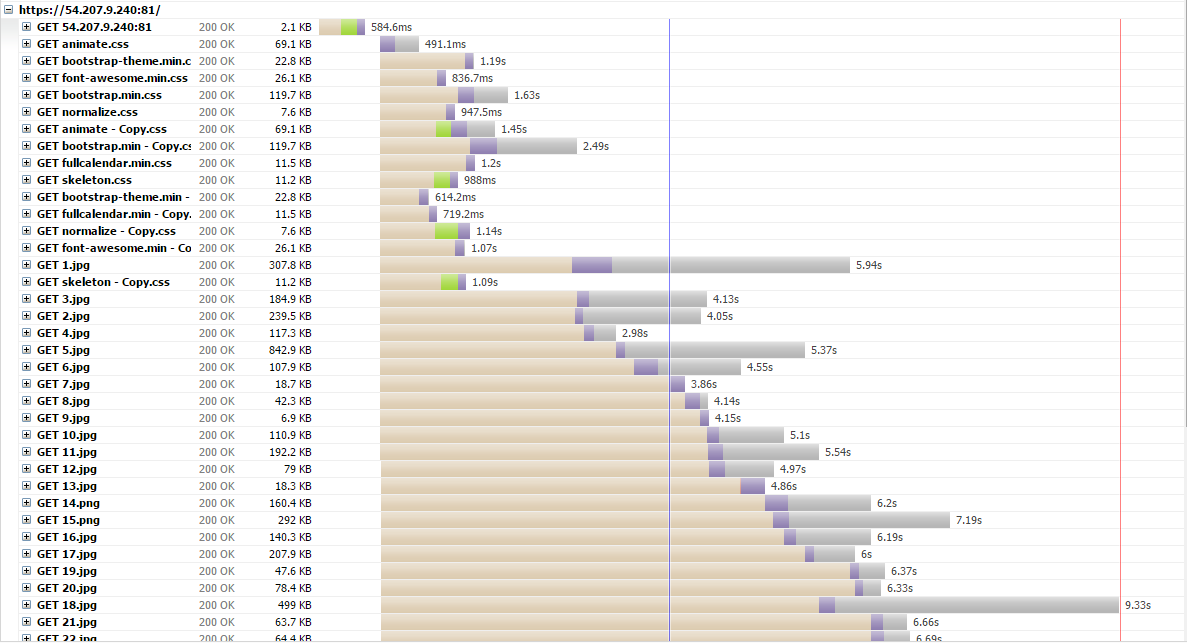
\includegraphics[width=1.5\textwidth]{./04-figuras/cascatas/separados_http11}
	\end{figure}
\end{landscape}

\begin{landscape}
	\begin{figure}[!htb]
    	\centering
	    \caption{Cascata ''Faça menos requisições HTTP'' - Arquivos separados - HTTP/2.}
	    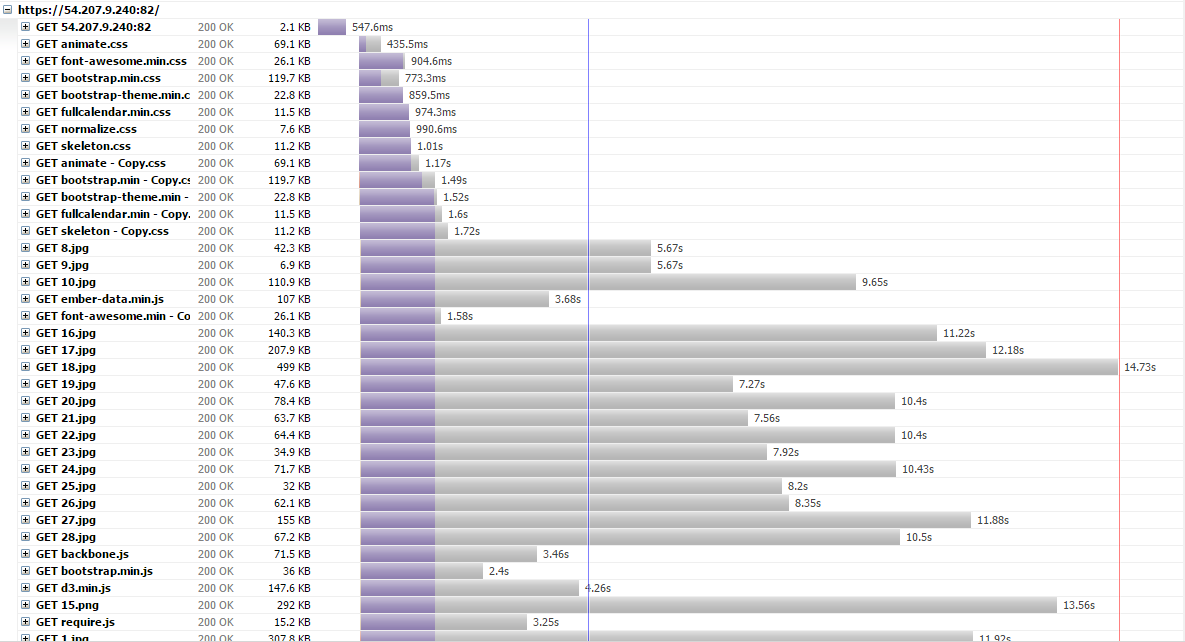
\includegraphics[width=1.5\textwidth]{./04-figuras/cascatas/separados_http2}
	\end{figure}
\end{landscape}

\begin{landscape}
	\begin{figure}[!htb]
    	\centering
	    \caption{Cascata ''Faça menos requisições HTTP'' - Arquivos concatenados - HTTP/1.1.}
    	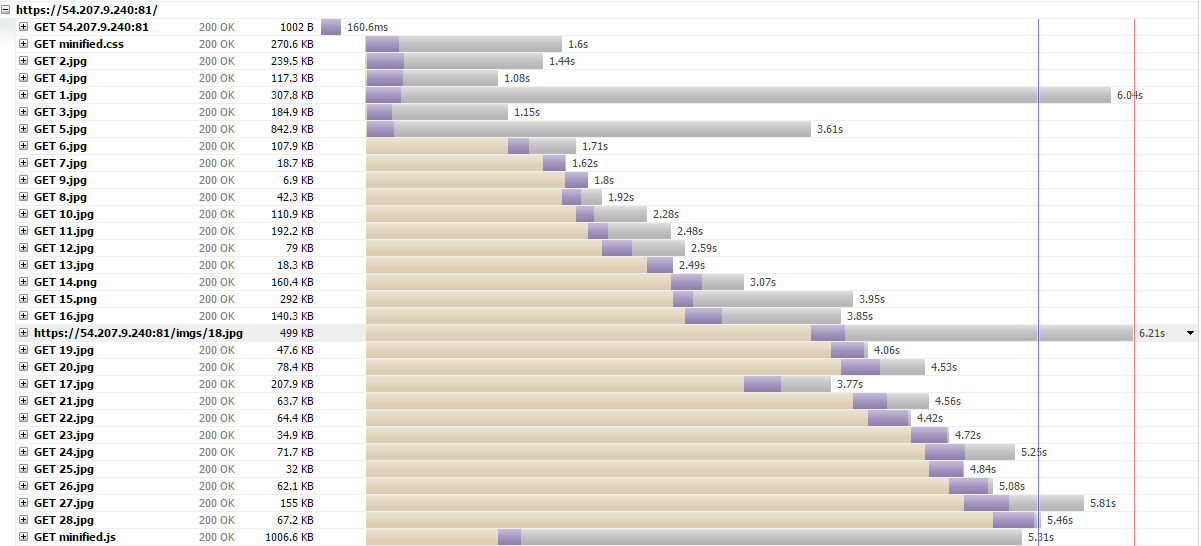
\includegraphics[width=1.5\textwidth]{./04-figuras/cascatas/concatenado_http11}
	\end{figure}
\end{landscape}

\begin{landscape}
	\begin{figure}[!htb]
    	\centering
	    \caption{Cascata ''Faça menos requisições HTTP'' - Arquivos concatenados - HTTP/2.}
	    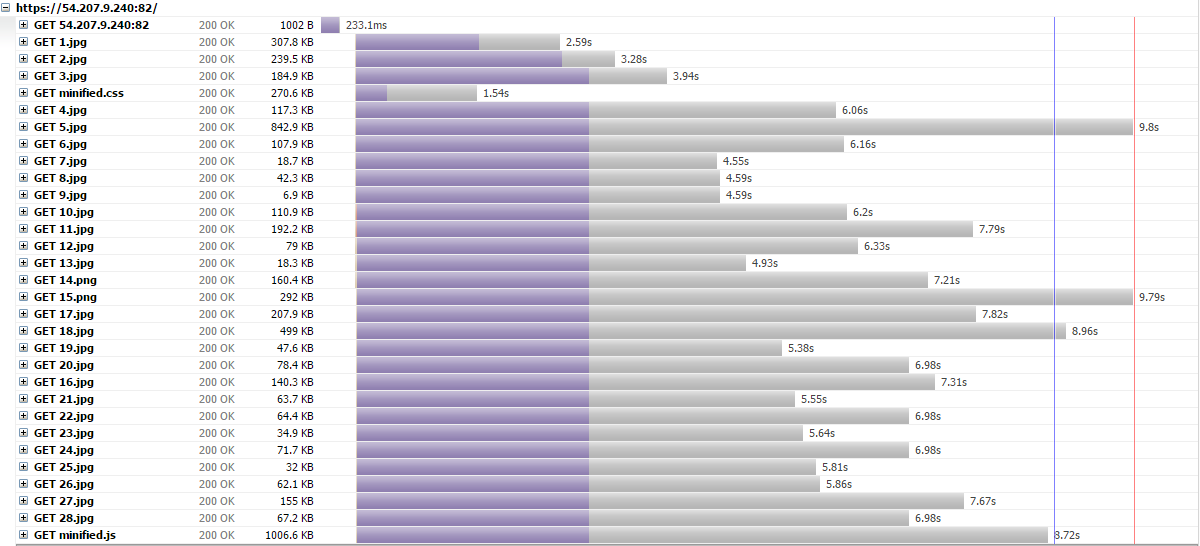
\includegraphics[width=1.5\textwidth]{./04-figuras/cascatas/concatenado_http2}
	\end{figure}
\end{landscape}

\begin{landscape}
	\begin{figure}[!htb]
    	\centering
	    \caption{Cascata ''Reduza o número de pesquisas DNS'' - Única CDN - HTTP/1.1.}
	    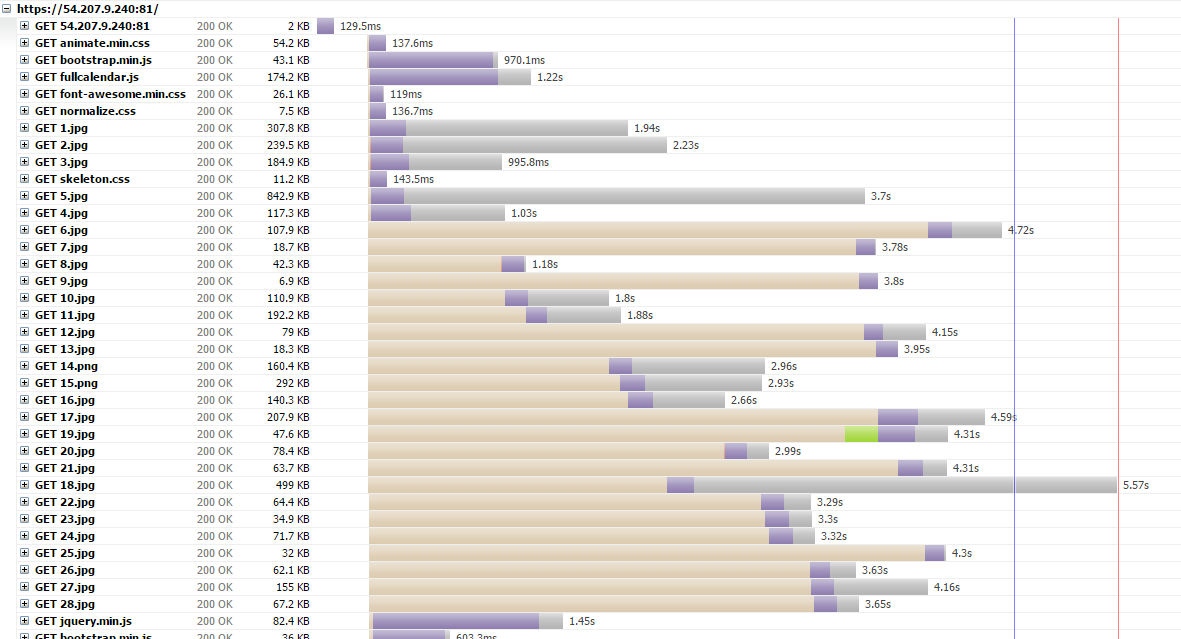
\includegraphics[width=1.5\textwidth]{./04-figuras/cascatas/single_http11}
	\end{figure}
\end{landscape}

\begin{landscape}
	\begin{figure}[!htb]
    	\centering
	    \caption{Cascata ''Reduza o número de pesquisas DNS'' - Única CDN - HTTP/2.}
	    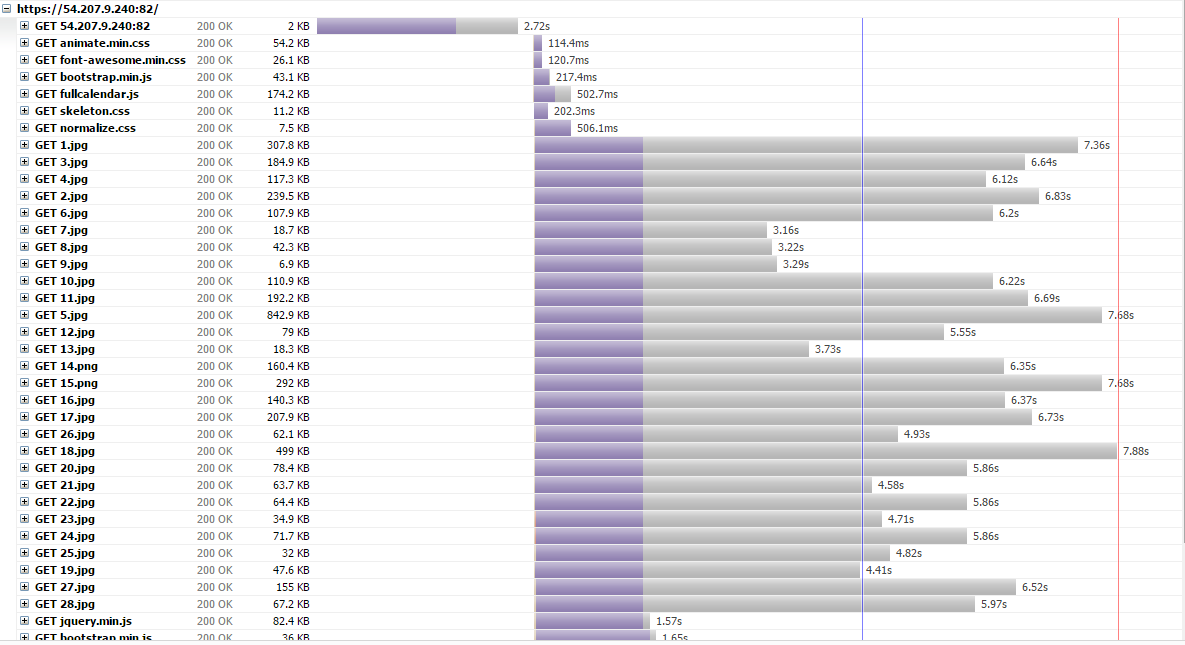
\includegraphics[width=1.5\textwidth]{./04-figuras/cascatas/single_http2}
	\end{figure}
\end{landscape}

\begin{landscape}
	\begin{figure}[!htb]
    	\centering
	    \caption{Cascata ''Reduza o número de pesquisas DNS'' - Multiplas CDN - HTTP/1.1.}
    	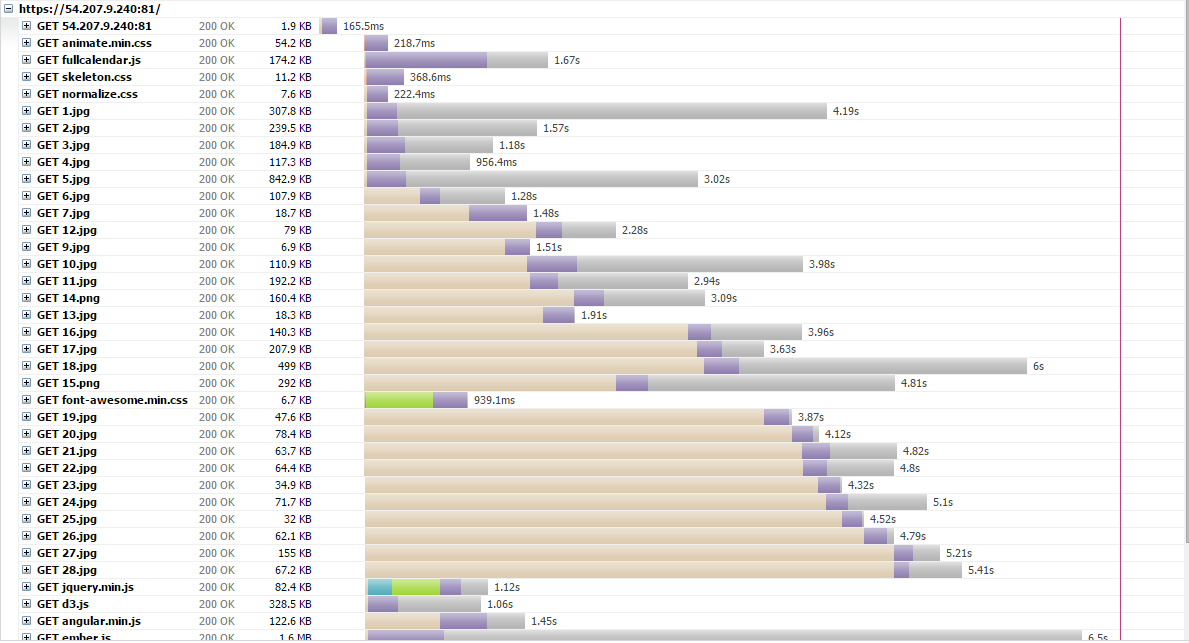
\includegraphics[width=1.5\textwidth]{./04-figuras/cascatas/multiple_http11}
	\end{figure}
\end{landscape}

\begin{landscape}
	\begin{figure}[!htb]
    	\centering
	    \caption{Cascata ''Reduza o número de pesquisas DNS'' - Multiplas CDNs - HTTP/2.}
	    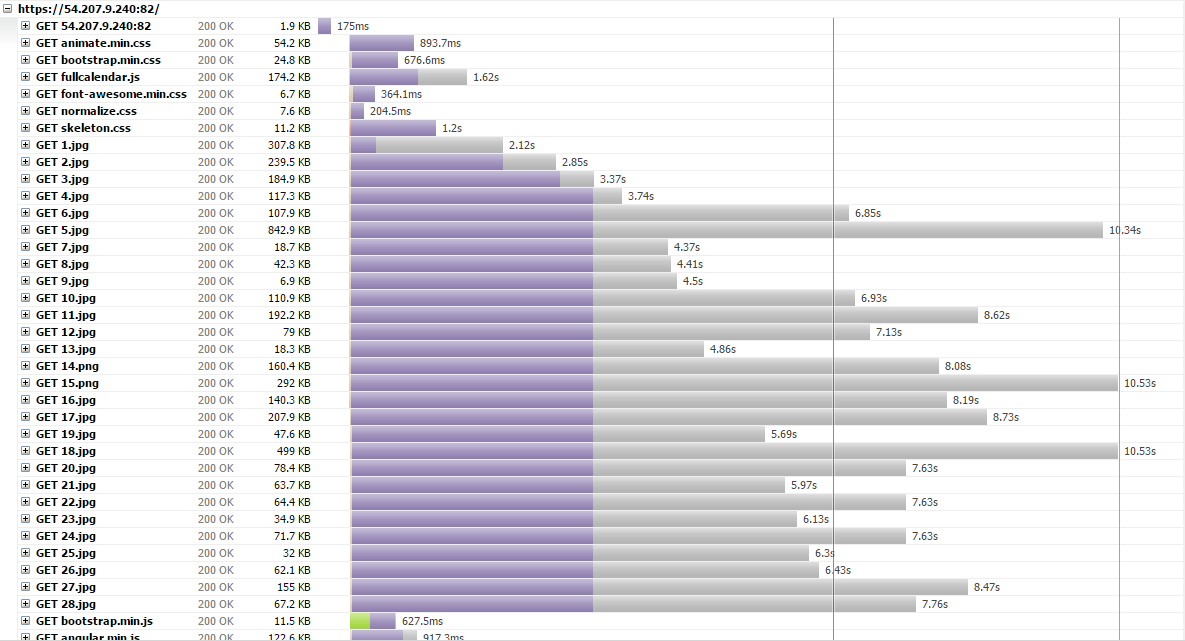
\includegraphics[width=1.5\textwidth]{./04-figuras/cascatas/multiple_http2}
	\end{figure}
\end{landscape}

\begin{landscape}
	\begin{figure}[!htb]
    	\centering
	    \caption{Cascata ''Quebrando domínios dominantes'' - 2 CDNs - HTTP/1.1.}
	    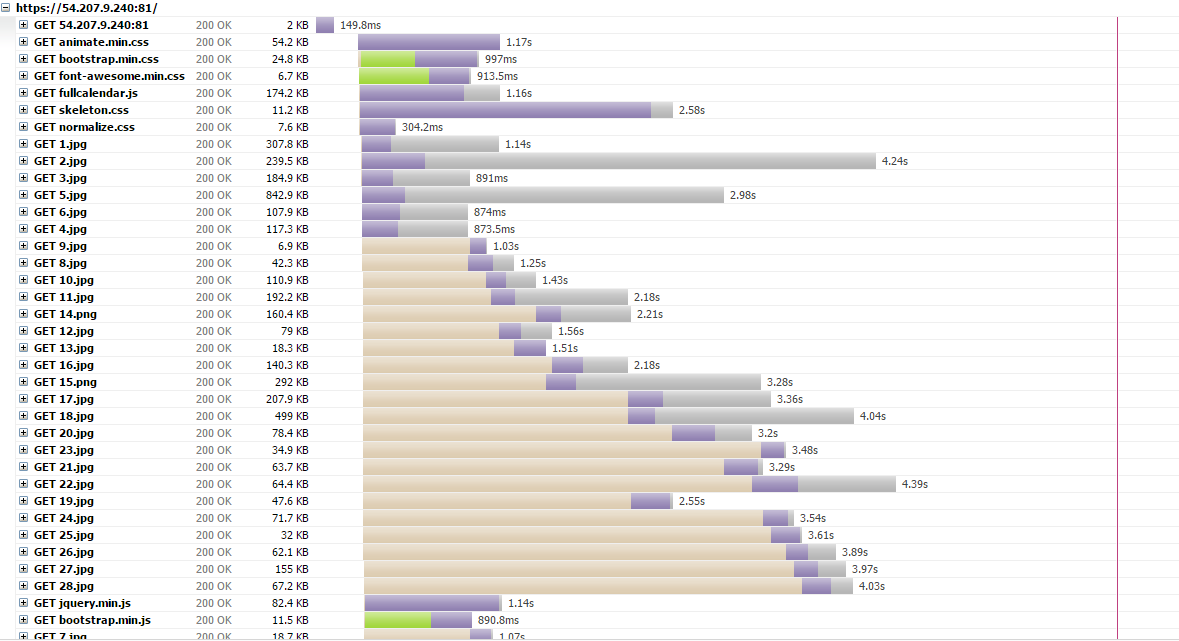
\includegraphics[width=1.5\textwidth]{./04-figuras/cascatas/2cds_http11}
	\end{figure}
\end{landscape}

\begin{landscape}
	\begin{figure}[!htb]
	    \centering
	    \caption{Cascata ''Quebrando domínios dominantes'' - 2 CDNs - HTTP/2.}
	    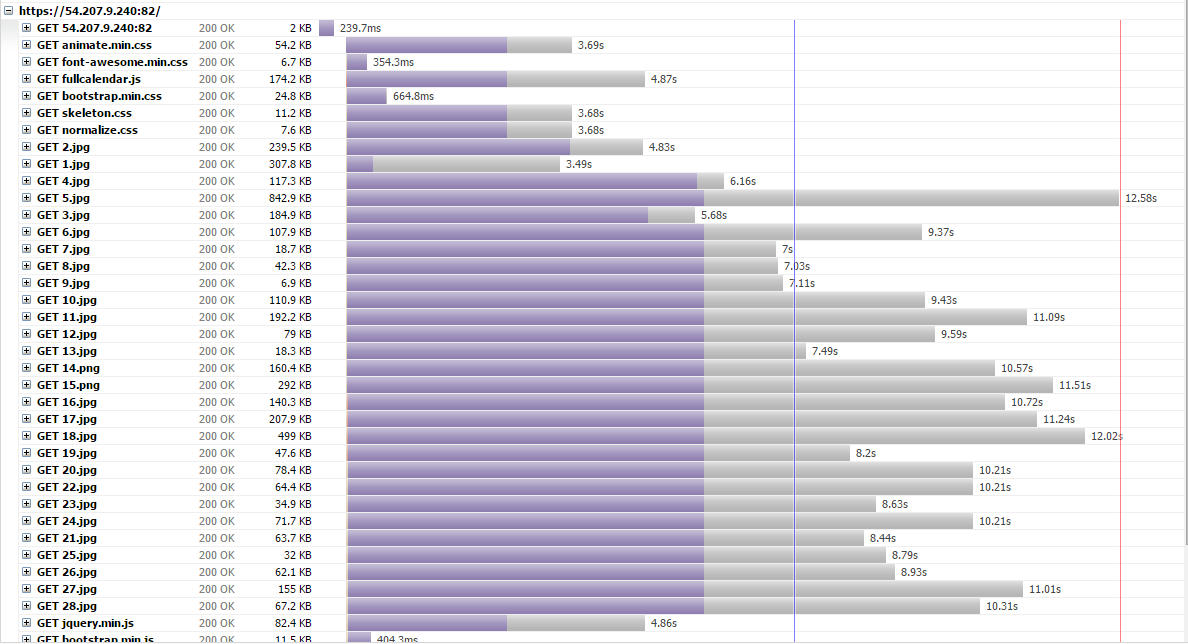
\includegraphics[width=1.5\textwidth]{./04-figuras/cascatas/2cds_http2}
	\end{figure}
\end{landscape}

\begin{landscape}
	\begin{figure}[!htb]
    	\centering
	    \caption{Cascata ''Quebrando domínios dominantes'' - 3 CDNs - HTTP/1.1.}
	    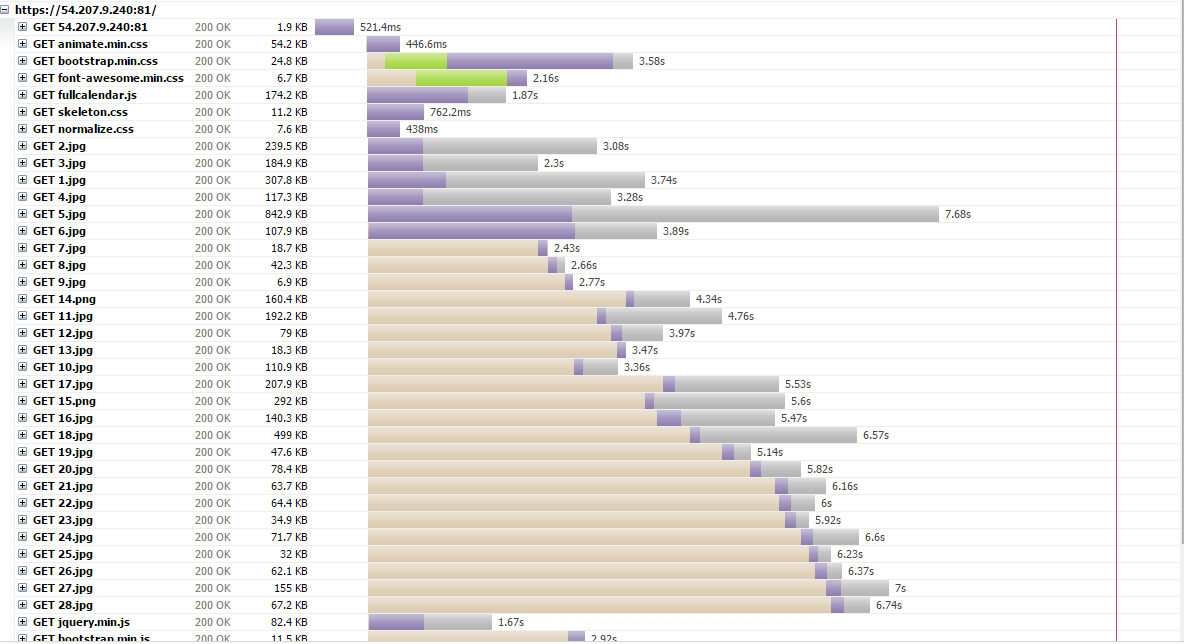
\includegraphics[width=1.5\textwidth]{./04-figuras/cascatas/3cds_http11}
	\end{figure}
\end{landscape}

\begin{landscape}
	\begin{figure}[!htb]
    	\centering
	    \caption{Cascata ''Quebrando domínios dominantes'' - 3 CDNs - HTTP/2.}
    	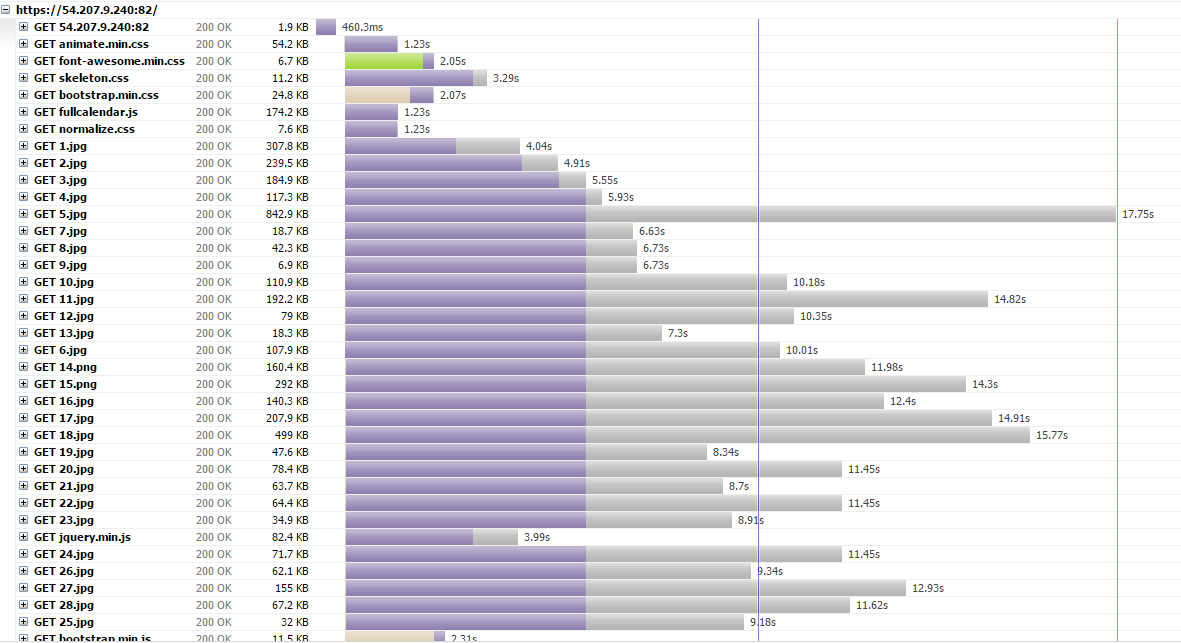
\includegraphics[width=1.5\textwidth]{./04-figuras/cascatas/3cds_http2}
	\end{figure}
\end{landscape}

\begin{landscape}
	\begin{figure}[!htb]
    	\centering
	    \caption{Cascata ''Template'' - HTTP/1.1.}
	    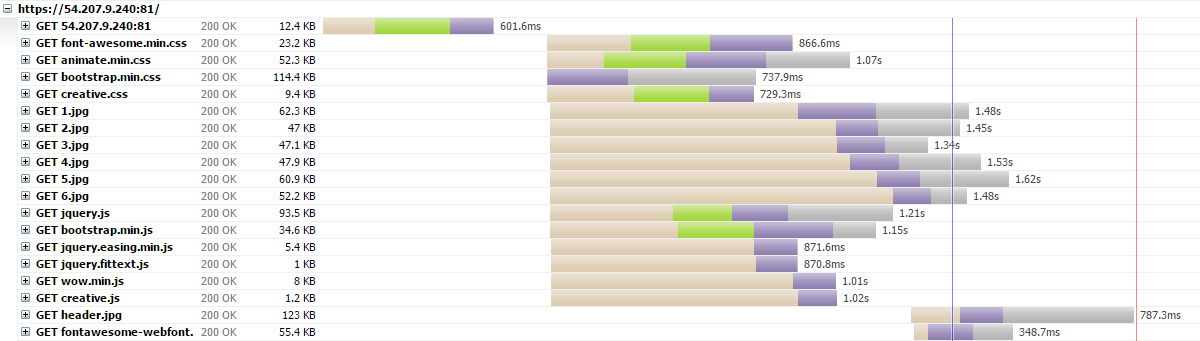
\includegraphics[width=1.5\textwidth]{./04-figuras/cascatas/template_http11}
	\end{figure}
\end{landscape}

\begin{landscape}
	\begin{figure}[!htb]
	    \centering
	    \caption{Cascata ''Template'' - HTTP/2.}
	    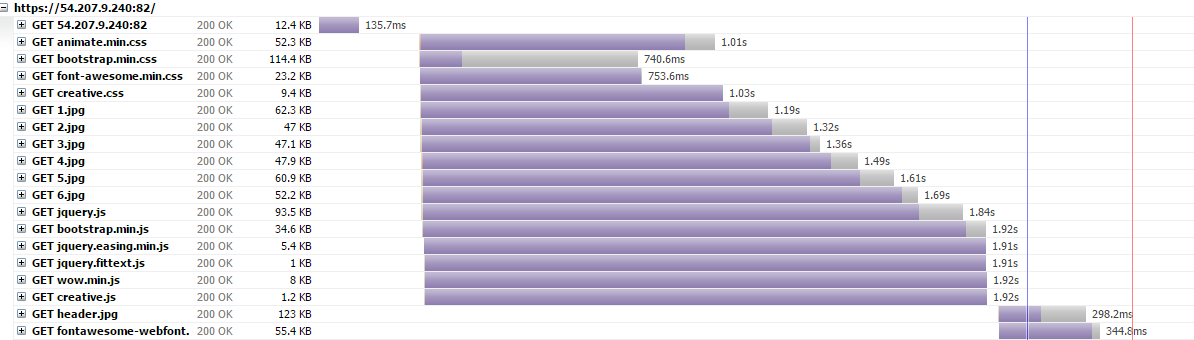
\includegraphics[width=1.5\textwidth]{./04-figuras/cascatas/template_http2}
	\end{figure}
\end{landscape}


\end{apendicesenv}